\newpage
\section{CPU scheduling}

So far we have talked about processes and threads: what they are, how to implement them, how to increase maximum speed, how to use libraries to implement them, etc.

Now we want to know the behavior of all this, how the operating system interacts and handles these activities.


\subsection{Basic Concepts}

We want to maximize CPU utilization obtained with multiprogramming. The tasks are only CPU burst and I/O burst: Process
execution consists of a cycle of CPU execution and I/O wait, in the same order.

The CPU burst distribution is of main concern.

\begin{figure}[htbp]
    \centering
    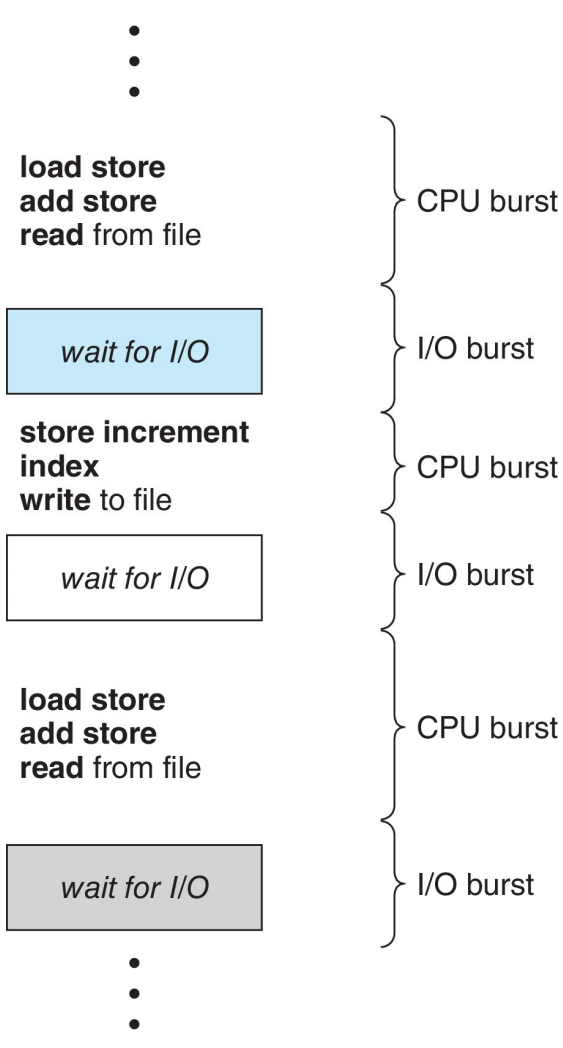
\includegraphics[width=0.35\linewidth]{img/CPU_BURST.png}
    
    
\end{figure}

So, if a programme  that performs sorting uses the CPU, but when it waits for some I/O the tasks does not use CPU and we want to pull it out from the CPU because others process want use it.


\paragraph{Histogram of CPU-burst Times}
Large number of short bursts and small number of longer bursts.
\begin{figure}[htbp]
    \centering
    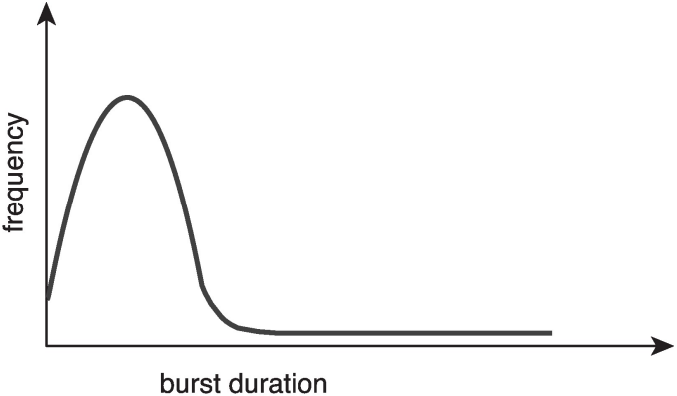
\includegraphics[width=0.4\linewidth]{img/vurst.png}
    
    
\end{figure}

\newpage
\subsection{CPU Scheduler}
The CPU Scheduler working to dispatching tasks to all the cores of the CPU. 

The CPU scheduler selects from among the processes in ready queue, and allocates a CPU core to one of them: Queue may be ordered in various ways.

\paragraph{}
So far, in fact when a task enters the CPU we do not have a method to kick it out and take another one from the ready queue an put it into the cpu, we waiting until it ends.

For this reasons CPU scheduling decisions may take place when a process:
\begin{enumerate}
    \item Switches from running to waiting state
    \item Switches from running to ready state
    \item Switches from waiting to ready
    \item Terminates
\end{enumerate}

For situations 1 and 4, there is no choice in terms of managing the
ready queue. Simply, a new process is taken from the queue.

For situations 2 and 3, however, there is a choice that is up to the
scheduler.

\begin{figure}[htbp]
    \centering
    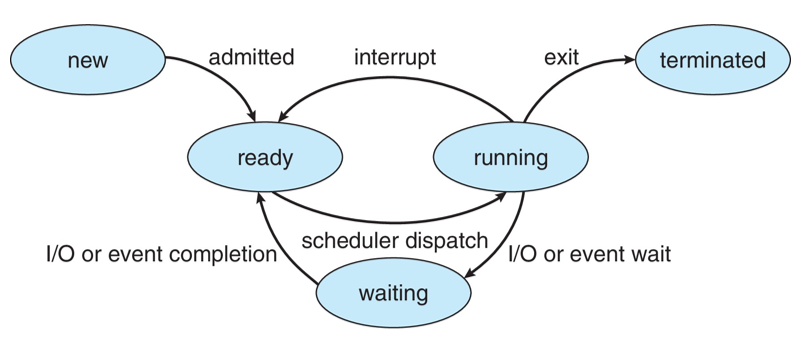
\includegraphics[width=0.65\linewidth]{img/process_state_diagram.png}
    \caption{Diagram of Process State}    
\end{figure}

\subsection{Preemptive and Nonpreemptive Scheduling}

Under \textbf{Nonpreemptive scheduling}, once the CPU has been
allocated to a process, the process keeps the CPU until it
releases it either by \textbf{terminating} or by switching to the \textbf{waiting
state}.

Otherwise, it is \textbf{preemptive}.

Thus, a process could theoretically keep it forever, or, before the OS recognizes this anomalous behavior
and kills it.

\paragraph{}
Virtually all modern operating systems including Windows, MacOS, Linux, and UNIX use preemptive scheduling algorithms.
This methods allows to set a priority to each tasks.

\subsubsection{Preemptive Scheduling and Race Conditions}

Preemptive scheduling can result in race conditions when data are
shared among several processes.

\paragraph{}

Consider the case of two processes that share data. While one
process is updating the data, it is preempted so that the second
process can run. The second process then tries to read the data,
which are in an inconsistent state (data consistency).

\begin{codeInC}
void myFunction(){
    int myID = thread;
    myID++;
}

\end{codeInC}

If it is nonpreemptive the function stuck into the cpu untill the function \verb|myFunction()| terminate (line: 5), otherwise if it is preemptive the CPU scheduler may stopped the execution at line 3 another process could execute the function and the two process have the same myID.

\paragraph{Note:} these problems happen only when one process writes and at
least another one tries to read it.
Read-only variables or atomic block will never have any kind of problems and can
be shared without issues.

\subsection{Dispatcher}
Assume that the CPU decided that a given task P1 has to be assigned to a core now running P0. Then what?

Dispatcher module gives control of the
CPU to the process selected by the CPU
scheduler; this involves:

\begin{itemize}
    \item Switching context;
    \item Switching to user mode;
    \item Jumping to the proper location in the user program to restart that program;
\end{itemize}

\begin{figure}[htbp]
    \centering
    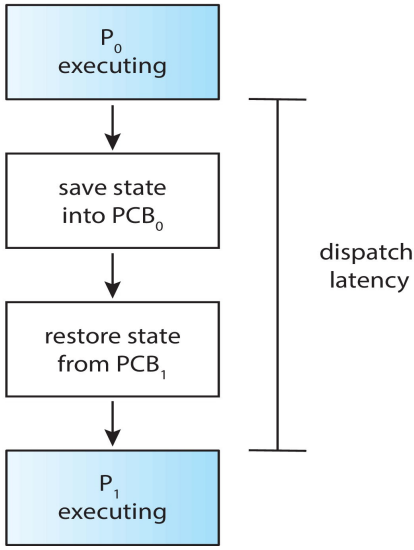
\includegraphics[width=0.3\linewidth]{img/dispacher.png}
    \caption{Dispatcher}    
\end{figure}

\textbf{Dispatch latency} – time it takes for the dispatcher to stop one process and start another running. The preemptive don't give nothing for free.

\subsection{Scheduling Criteria}

There are some parameters that the CPU scheduler could optimize, but not all of them because some of some of them conflict.

\begin{itemize}
    \item \textbf{CPU utilization} - keep the CPU as busy as possible;
    \item \textbf{Throughput} – \# of processes that complete their execution per time unit;
    \item \textbf{Turnaround time} – amount of time to execute a particular process;
    \item \textbf{Waiting time} – the amount of time a process has been waiting in the ready queue;
    \item \textbf{Response time} – amount of time it takes from when a process enters the ready queue to when it gets into the CPU the first time. 
\end{itemize}

The first two are connected. 

\newpage
\section{Scheduling Algorithms}

\subsection{FCFS}

\begin{figure}[htbp]
    \centering
    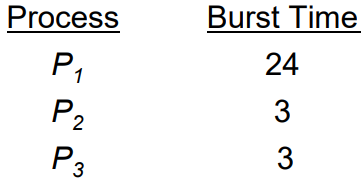
\includegraphics[width=0.25\linewidth]{img/FCFS.png}
    \caption{First- Come, First-Served}    
\end{figure}

The First-Come, First-Served Scheduling is non preemptive: once assigned, a process finishes is
execution.

\paragraph{}

\textbf{Waiting time} for P1, P2, P3: 0, 24, 27;
\textbf{Average waiting time}: $(0 + 24 + 27)/3 = 17$.

\paragraph{}
But if the processes arrive in the order: P2,P3,P1, we obtain other number:

\textbf{Waiting time} for P1, P2, P3: 6, 0, 3;
\textbf{Average waiting time}: $(6 + 0 + 3)/3 = 3$.

Much better than previous case. This case is called \textbf{convoy effect} - short process behind long process.

\subsection{SJF}
Shortest-Job-First Scheduling or, better, shortest-next-CPU-burst. This method minimize the waiting time.

\paragraph{}
Associate with each process the length of its next CPU burst, but there is a big problem: How do we determine the length of the next CPU burst?

\begin{itemize}
    \item Could ask the user:  unfeasible, introduces delays;
    \item Estimate but how?
\end{itemize}


\subsubsection{Determining Length of Next CPU Burst}
Can be done by using the length of previous CPU bursts (of the same task), using exponential averaging:

\begin{equation}
    \tau_{n+1} = \alpha t_n + (1+\alpha)\tau_n
\end{equation}

where:
\begin{itemize}
    \item $t_n$: actual length of the $n^{th}$ CPU burst;
    \item $\tau_{n+1}$: predicted value for the next CPU burst
    \item $\alpha$ set to 0.5, $ 0 \leq \alpha \leq 1$ 
\end{itemize}

\newpage

\begin{figure}[htbp]
    \centering
    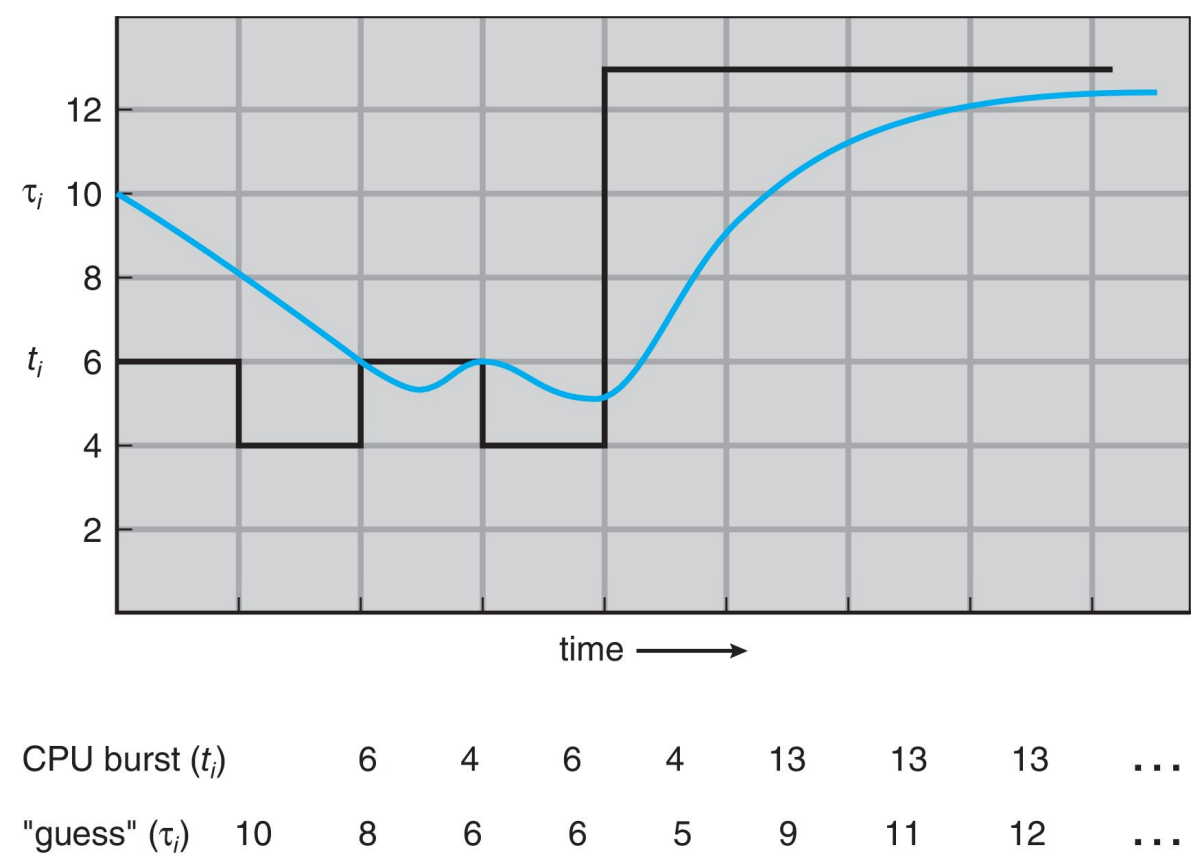
\includegraphics[width=0.55\linewidth]{img/prediction.png}
    \caption{Prediction vs Actual CPU Burst}    
\end{figure}


This method is precise if the CPU burst does not change a lot.

\subsection{SRT}

The Shortest-Remaining-Time-first is the preemptive version of SJN. Whenever a new process arrives in the ready queue, the
decision on which process to schedule next is redone using the SJN algorithm.

Is SRT more “optimal” than SJN in terms of the minimum average waiting time for a given set of processes?


\begin{figure}[htbp]
    \centering
    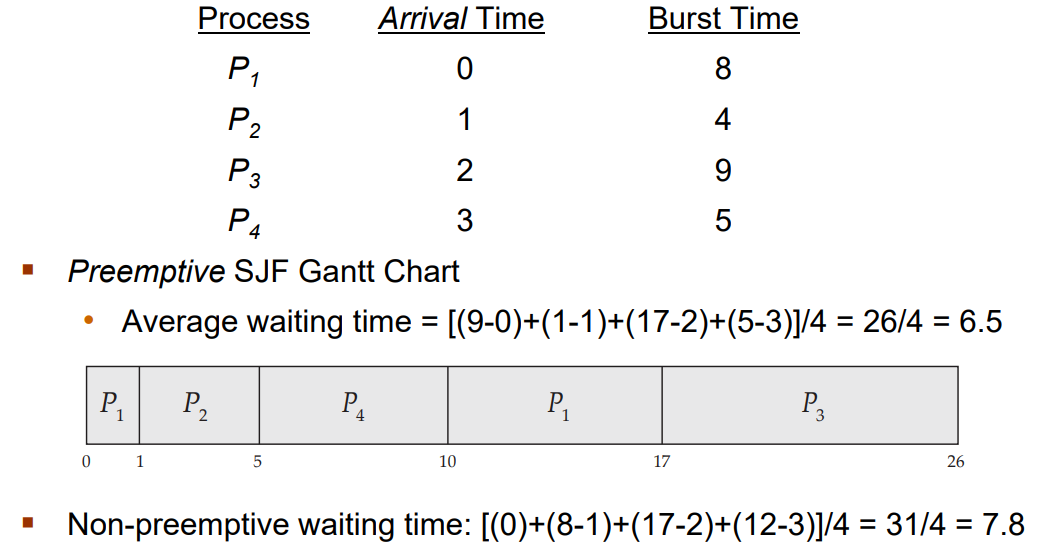
\includegraphics[width=0.65\linewidth]{img/SRTF.png}
  
\end{figure}

\newpage
\subsection{Round Robin}

Each process gets a small unit of CPU time (\textbf{time quantum} or \textbf{time slice} q), usually 10-100 milliseconds. After this time has elapsed, the process is preempted and added to the end of the ready queue.

If there are n processes in the ready queue and the time quantum
is q, then each process gets 1/n of the CPU time in chunks of at
most q time units at once. No process waits more than \textbf{(n-1)q}
time units.

\paragraph{}
Timer interrupts every quantum to schedule next process.

\paragraph{Performance:}
\begin{itemize}
    \item [] q large: FIFO (FCFS);
    \item [] q small: RR.
\end{itemize}

\paragraph{NOTE:} the q must be larger with respect to context switch, otherwise overhead is to high, there will be no execution, just context switches after context switches (useless).


\subsubsection{RR vs FCFS}


\begin{figure}[htbp]
    \centering
    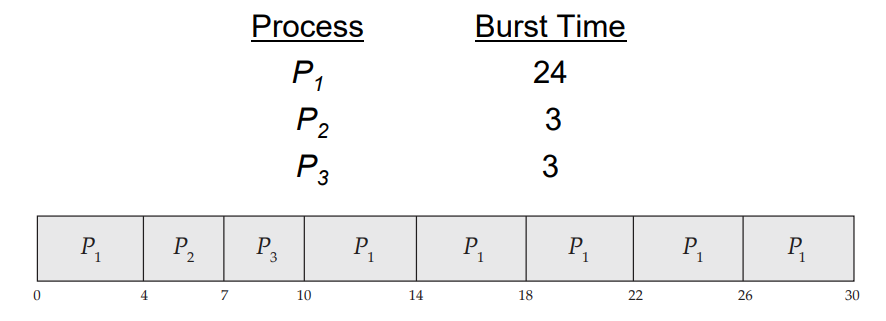
\includegraphics[width=0.6\linewidth]{img/RR.png}    
    
\end{figure}

Typically, higher average turnaround than SJF, but better \textbf{response}:
\begin{itemize}
    \item[] Waiting Average = (6 + 4 + 7) / 3 = 5.7
    \item[] Turnaround = (30 + 3 + 3) / 3 = 12
    \item[] Response = (4 + 7 + 10) / 3 = 7 
\end{itemize}

\begin{figure}[htbp]
    \centering
    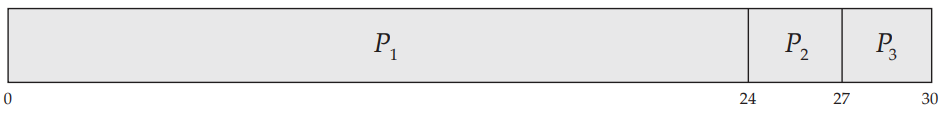
\includegraphics[width=0.6\linewidth]{img/FSCS_VSR.png}   
    
\end{figure}

\begin{itemize}
    \item[] Waiting Average =  (0 + 24 + 27) / 3 = 17
    \item[] Turnaround =  (24 + 3 + 3) / 3 = 10
    \item[] Response = (0 + 24 + 27) / 3 = 17 
\end{itemize}

\subsubsection{Turnaround Time Varies With The Time Quantum}

Rule of Thumb: 80\% of CPU bursts should be shorter than q.

\paragraph{Example: } processes P1, P2, P3, P4 with respectively time 6, 3, 1, 7; a good q could be 6.

\newpage
\section{Priority Scheduling}

A priority number (integer) is associated with each process. The CPU  is allocated to the process with the highest priority, smaller integer $\equiv$ highest priority.

\begin{itemize}
    \item Preemptive: the scheduler kick the task out the CPU for some reasons;
    \item Non-preemptive: the scheduler must not kick the task out the CPU unless it waiting for an I/O.
\end{itemize}

But not all the tasks are the same, in fact there are users threads and kernel threads. This latter should not be blocked by the users threads.

\paragraph{}
\textbf{SJV} is a priority scheduling where priority is the inverse of the predicted next CPU bust. Regardless to all the algorithm chose the tasks that have the higher priority, it means it have the lower CPU burst time.


But there is a problem:

\begin{itemize}
    \item[] \textbf{Starvation} - low priority tasks may never execute
\end{itemize}

The solution of this problem is called:

\begin{itemize}
    \item[] \textbf{Aging} - if tasks does not execute in n-time, its priority (age) is increased, this process is repeated until the execution arrives. The more a process remains in the ready queue, the more his priority (age) increase.
\end{itemize}

e.g. if the tasks is in the ready queue for 4 CPU burst, I increase its priority.

\subsubsection{Example of Priority Scheduling}

\begin{figure}[htbp]
    \centering
    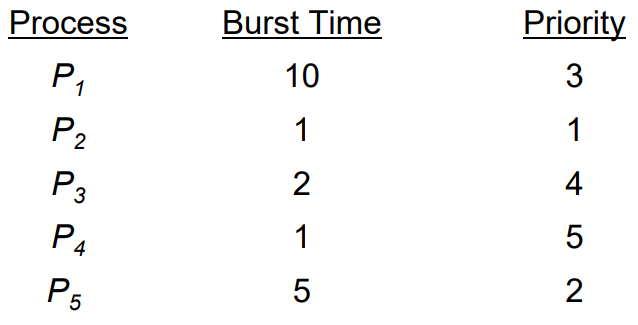
\includegraphics[width=0.4\linewidth]{img/priority_sched.png}  
\end{figure}

The scheduler in this situation does not take care about the CPU burst time, it look at the priority of the process.

\begin{figure}[htbp]
    \centering
    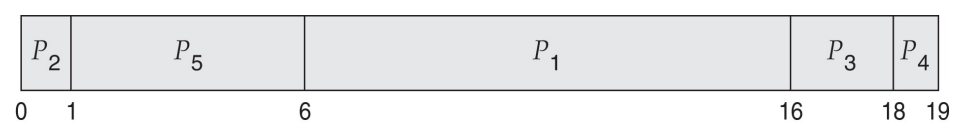
\includegraphics[width=0.65\linewidth]{img/gantt.png}
\end{figure}

This priority scheduling has an average waiting time of 8.2. But the burst of CPU of course is important for improving average waiting.
\paragraph{}

But if the processes are the same priority? There is some mechanism that allow to chose one or the other tasks, we can chose different type of scheduling algorithms:

\begin{itemize}
    \item Priority scheduling with Round-Robin - same priority, the tasks to execute first is chose by the random algorithm;
    \item Priority scheduling with FCFS - same priority, the tasks to execute first is chose by the first come first served algorithm;
    \item Priority scheduling with SJF - same priority, the tasks to execute first is chose by shortest jobs first algorithm;
    \item Other.
\end{itemize}

\begin{figure}[htbp]
    \centering
    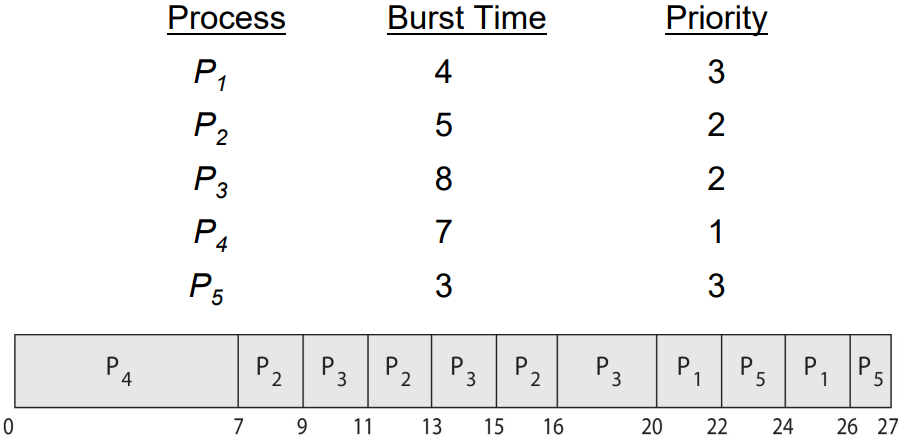
\includegraphics[width=0.5\linewidth]{img/PSWRR.png}
    \caption{Priority Scheduling w/ Round-Robin}    
\end{figure}

\section{Scheduling in using multiple queues}

Having different priority queues for all the priority level in the OS, allow to implement different scheduling algorithms for each queues to decide witch tasks going to be execute first.

\subsection{Multilevel queue}
Multilevel queue scheduler defined by the following parameters:

\begin{itemize}
    \item Number of queues;
    \item Scheduling algorithms for each queue;
    \item Method used to determine which queue a process will enter;
    \item when that process needs service;
    \item Scheduling among the queues.
\end{itemize}


With priority scheduling, have separate queues for each priority.

\begin{figure}[htbp]
    \centering
    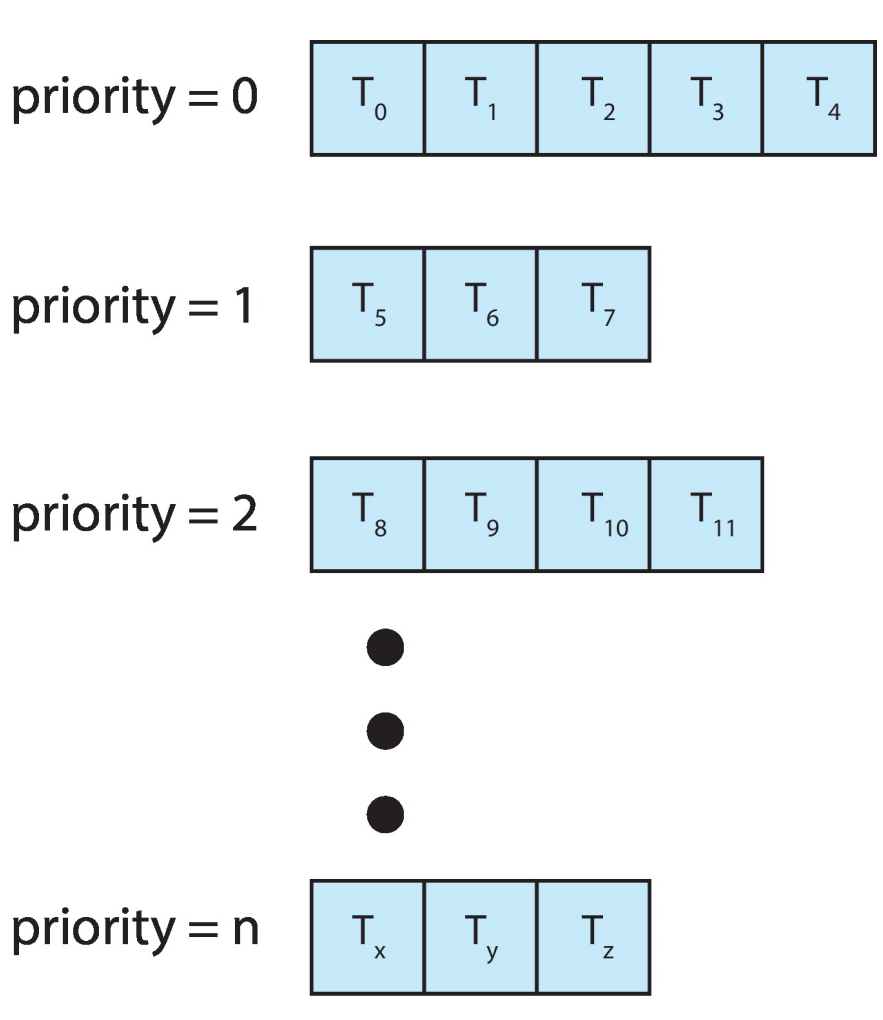
\includegraphics[width=0.35\linewidth]{img/multileve_queue.png}
    \caption{Multilevel queue}    
\end{figure}

Aging can be implemented using multilevel feedback queue.

\paragraph{Example of multilevel feedback queue: } we look at the CPU bust and not to the priority.

\paragraph{}
Three queues:
\begin{itemize}
    \item Q0 – RR with time quantum 8 milliseconds
    \item Q1 – RR time quantum 16 milliseconds
    \item Q2 – FCFS
\end{itemize}

\newpage
Scheduling:  A new process enters queue Q0 which is served in RR

\begin{itemize}
    \item[--] When it gains CPU, the process receives 8 milliseconds
    \item[--] If it does not finish in 8 milliseconds, the process is moved to queue Q1
\end{itemize}

At Q1 job is again served in RR and receives 16 additional milliseconds, if it still does not complete, it is preempted and moved to queue Q2.

\begin{figure}[htbp]
    \centering
    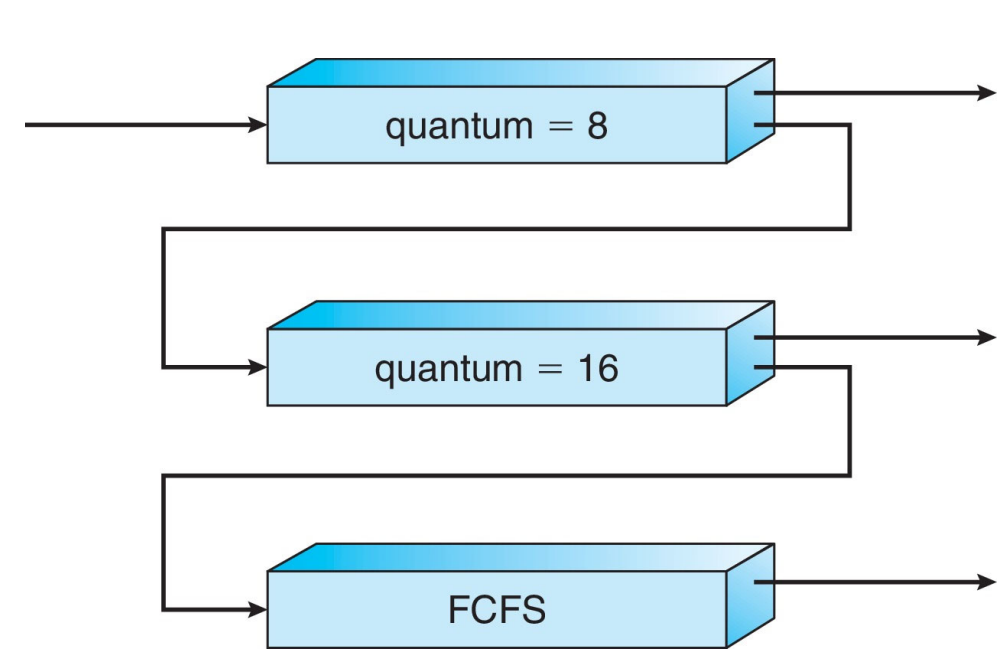
\includegraphics[width=0.45\linewidth]{img/multilever_queue.png}
\end{figure}

\subsection{Scheduling in multiprocessor systems}

CPU scheduling more complex when multiple CPUs are available, in fact multiprocess may be any one of the following architectures:

\begin{itemize}
    \item Multicore CPUs
    \item Multithreaded cores - the OS think to have double core 
    \item Heterogeneous multiprocessing
\end{itemize}

When you buy new processor on the box is written: this processor have L1, L2 and L3 cache. It means that the L1 cache is the private cache of the single core, this is divide in 2, L2 is the cache shared by the core, and the L3 cache is the cache shared by all core.

\subsubsection{Symmetric multiprocessing}
Symmetric multiprocessing (SMP) is where each processor is self scheduling.

\begin{itemize}
    \item All threads may be in a common ready queue (a) - more easier to implement, all tasks occupy the uncommitted core
    \item Each processor may have its own private queue of threads (b) - faster in context-switching, virus attack only one core
\end{itemize}


\begin{figure}[htbp]
    \centering
    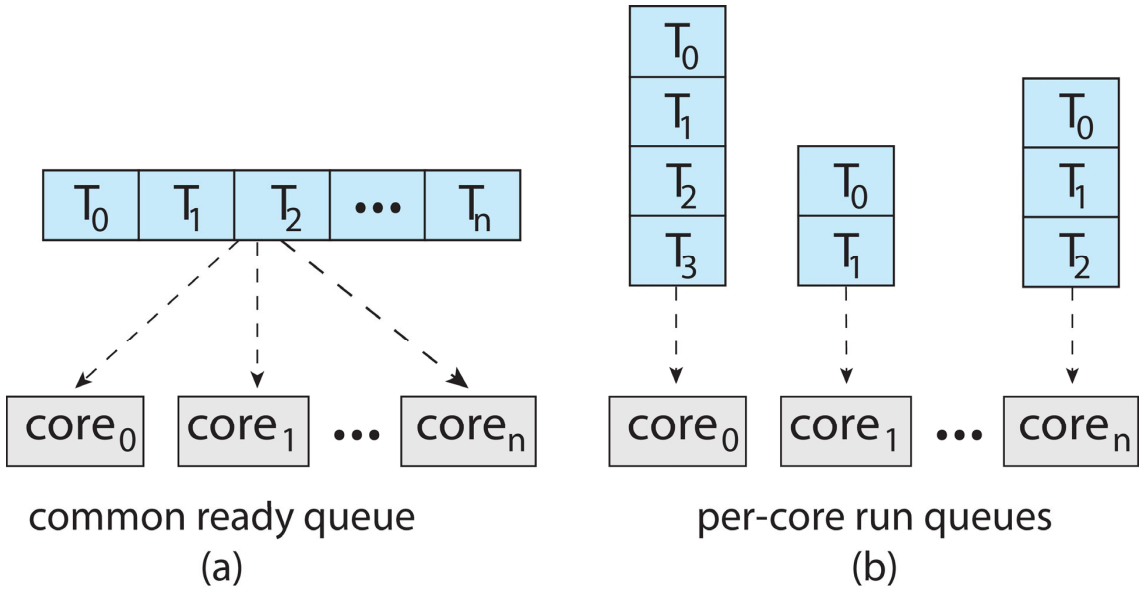
\includegraphics[width=0.55\linewidth]{img/SMP.png}   
    
\end{figure}


\subsection{Multi-core Processors}
Recent trend to place multiple cores on same physical chip, this approach is faster and consumes less power.

Multiple threads per core (virtual cores) also growing:

\begin{itemize}
    \item Takes advantage of memory stall to make progress on another thread while memory retrieve happens
    \item Each core has > 1 hardware threads
    \item If one thread has a memory stall, switch to another thread!
\end{itemize}

for those reason the L1 is divide in 2 or more area, witch each contains the data to another thread.

\begin{figure}[htbp]
    \centering
    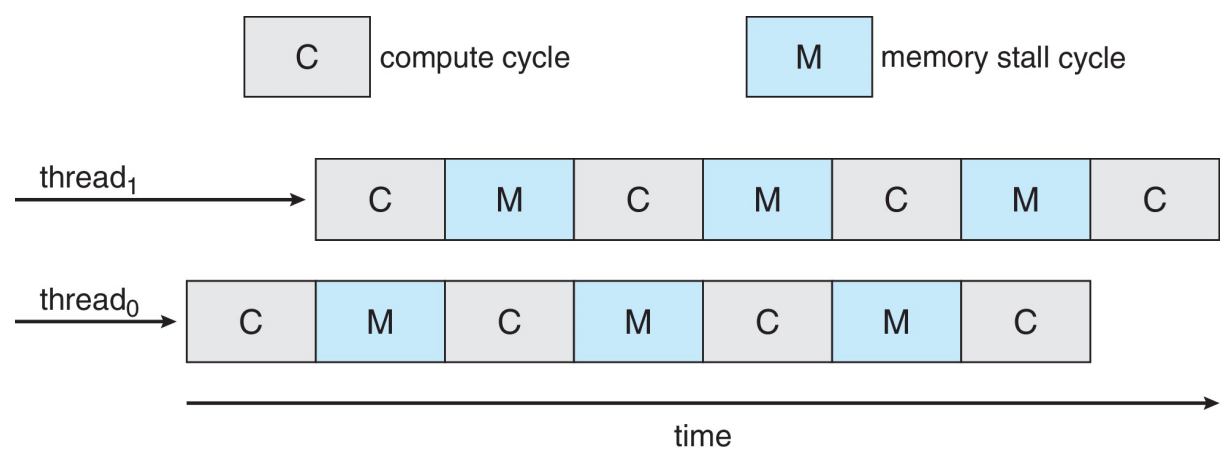
\includegraphics[width=0.6\linewidth]{img/memory_stall.png}   
    
\end{figure}

Chip-multithreading (CMT)
assigns each core multiple
hardware threads. (Intel refers
to this as hyperthreading.)

E.g. On a quad-core system with 2
hardware threads per core, the
operating system sees 8 logical
processors or virtual core.


\begin{figure}[htbp]
    \centering
    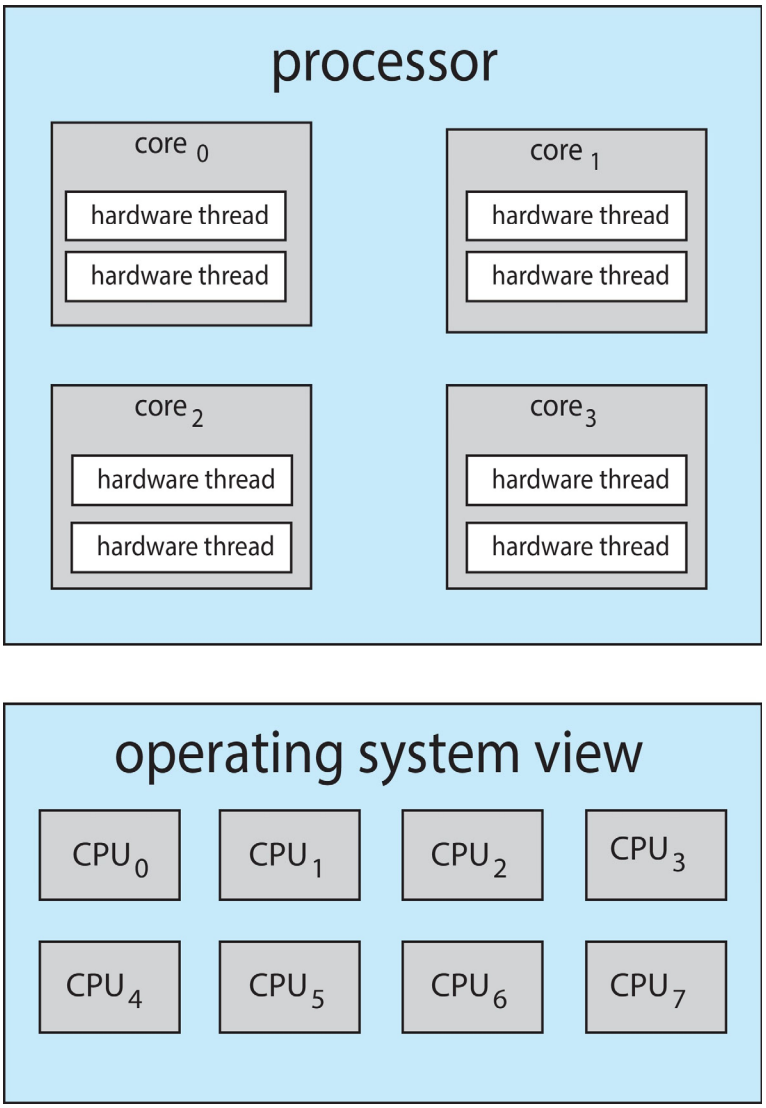
\includegraphics[width=0.35\linewidth]{img/hyperthreading.png}
    \caption{Chip-multithreading}    
\end{figure}

Also there are two level of scheduling:

\begin{enumerate}
    \item The operating system deciding which software thread to run on a logical CPU
    \item Each core decides which hardware thread to run on the physical core.
\end{enumerate}

\begin{figure}[htbp]
    \centering
    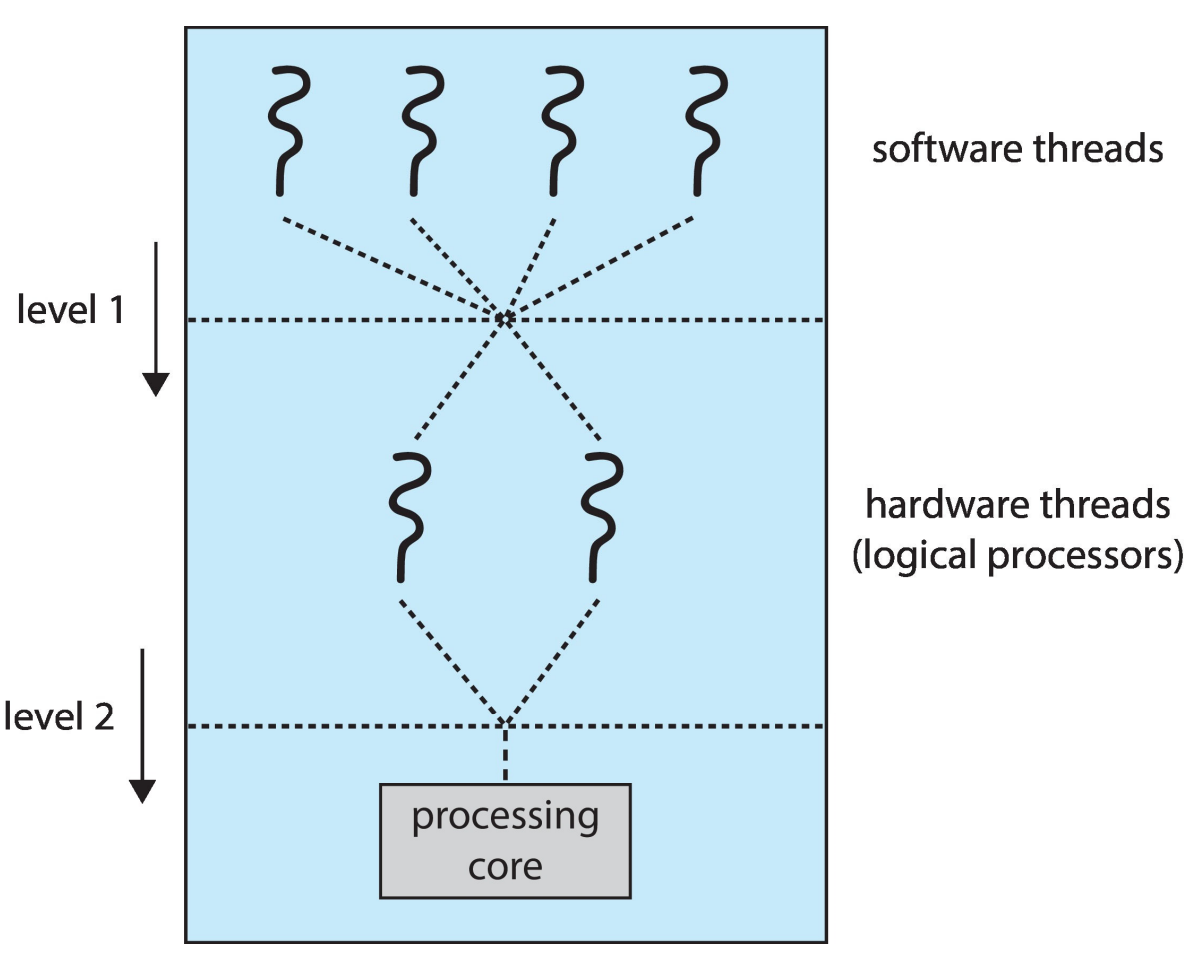
\includegraphics[width=0.5\linewidth]{img/level_thread.png}    
    
\end{figure}

\newpage
\subsubsection{Processor Affinity}
When a thread has been running on one processor, the cache contains some information and data and if the process return into the CPU it take the previous data from cache, this benefit in term of latency. We refer to this as a thread having affinity for a processor (i.e.
“processor affinity”).


\paragraph{}
Load balancing may affect processor affinity as a thread may be moved
from one processor to another to balance loads, yet that thread loses
the contents of what it had in the cache of the processor it was moved
off of.


\begin{itemize}
    \item \textbf{Soft affinity} – the operating system attempts to keep a thread running on the same processor, but no guarantees
    \item \textbf{Hard affinity }– allows a process to specify a set of processors it may run on.
\end{itemize}

\newpage
\section{Real time CPU scheduling}

For some reason, the tasks required to be execute in a specific time, or in real-time, e.g. ABS, train tracking and so on. They can present obvious challenges, there are two way to implement this functionality:

\begin{itemize}
    \item \textbf{Soft real-time systems} – Critical real-time tasks have the highest priority, but no guarantee as to when tasks will be scheduled;
    \item \textbf{Hard real-time systems} – task must be serviced by its deadline
\end{itemize}

\subsection{Latencies}
\textbf{Event latency} – the amount of time that elapses from when an event occurs to when it is serviced. There are two tipes of latencies affect performance: 

\textbf{Interrupt latency} – time from arrival of interrupt to start of routine that services interrupt
\textbf{Dispatch latency }– time for schedule to take current process off CPU and switch to another


\begin{figure}[htbp]
    \centering
    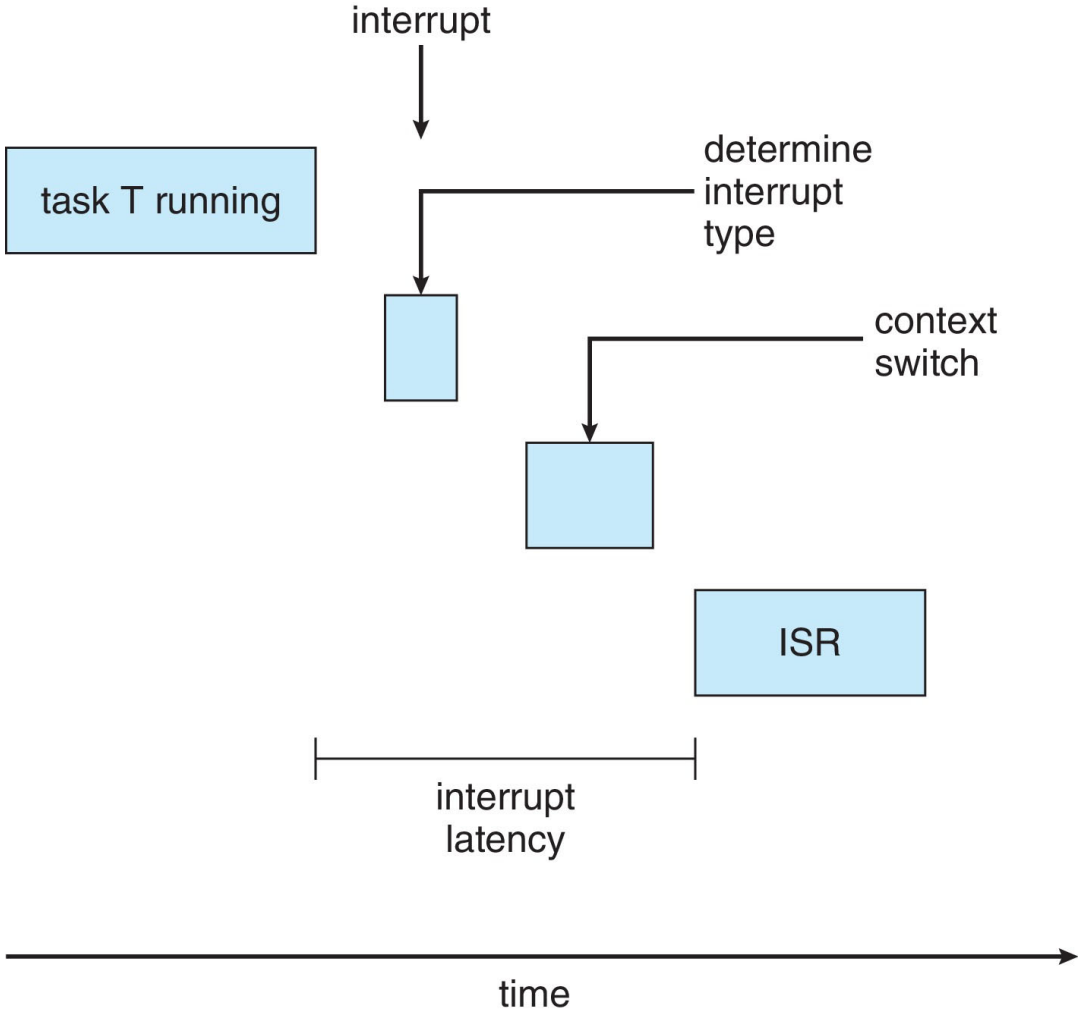
\includegraphics[width=0.45\linewidth]{img/latency.png}
    
    
\end{figure}


\subsection{Priority-based Scheduling}

For real-time scheduling, scheduler must support preemptive, prioritybased scheduling. But only guarantees \textbf{soft real-time}.

For hard real-time must also provide ability to meet \textbf{deadlines}.
\paragraph{}
Processes have new characteristics: \textbf{periodic} ones require CPU at constant intervals; this process has:

\begin{itemize}
    \item processing time t;
    \item deadline d;
    \item period p.
\end{itemize}

Rate of periodic task is 1/p


\begin{figure}[htbp]
    \centering
    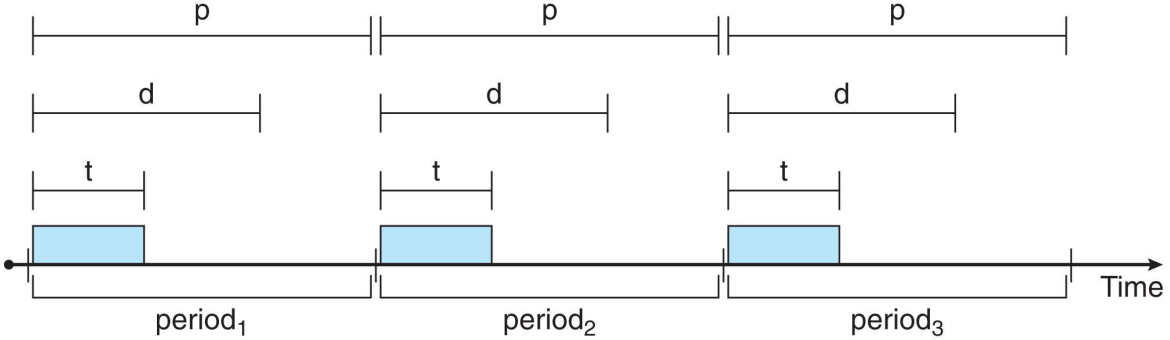
\includegraphics[width=0.75\linewidth]{img/priority_base.png}   
    
\end{figure}

\subsubsection{Rate Monotonic Scheduling (RMS)}
The priority is assigned based on the inverse of its period, priority = 1/period.

\begin{itemize}
    \item[] Shorter periods = higher priority;
    \item[] Longer periods = lower priority.
\end{itemize}

\paragraph{Example: } P1 is assigned a higher priority than P2, P1 has deadline 50, P2 has deadline 100

\begin{figure}[htbp]
    \centering
    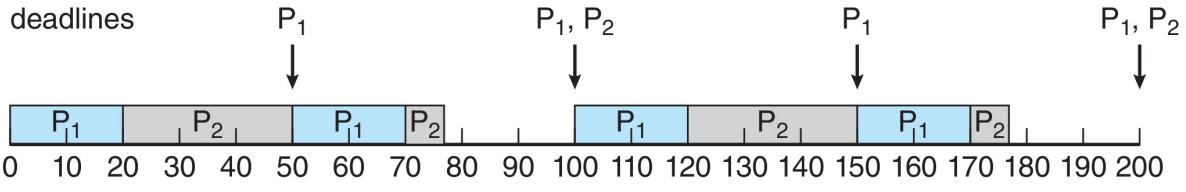
\includegraphics[width=0.7\linewidth]{img/RMP.png}
    
\end{figure}

RMS in not optimal solution, P1 is far from its deadline, but P2 is less far from its deadline. 

\subsubsection{Earliest Deadline First Scheduling (EDF)}

In this case the priorities are assigned according to deadlines:

\begin{itemize}
    \item[] The earlier the deadline, the higher the priority
    \item[] The later the deadline, the lower the priority
\end{itemize}


\begin{figure}[htbp]
    \centering
    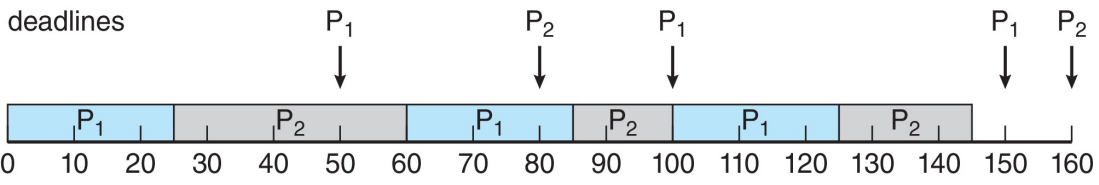
\includegraphics[width=0.7\linewidth]{img/EDF.png}
    
    
\end{figure}

All of this type of scheduling algorithms must have the minimum requirements of core numbers.

\newpage
\section{OS scheduling examples}

\subsection{Linux Scheduling in Version 2.6.23+}

The Linux scheduling is based on Completely Fair Scheduler (CFS). It is composed of:

\paragraph{Scheduling classes: } each tasks has specific priority, scheduler picks highest priority task in highest scheduling class, rather than quantum based on fixed time allotments, based on proportion of CPU time.

Two scheduling classes included, others can be added:

\begin{enumerate}
    \item default;
    \item real-time.
\end{enumerate}

\paragraph{Virtual run time:} CFS scheduler maintains per task virtual run time in variable \verb|vruntime|. Associated with decay factor based on priority of task – lower priority
is higher decay rate, normal default priority yields virtual run time = actual run time.

\paragraph{}
To decide next task to run, scheduler picks task with lowest virtual run time. But how to implement all of this?

\paragraph{}
To decide witch tasks to run the CFS looks at the \verb|vruntime|, the smartest way to implement this is to see the ready queue like a btree. In this way you have the smallest value always in the same position.


\begin{figure}[htbp]
    \centering
    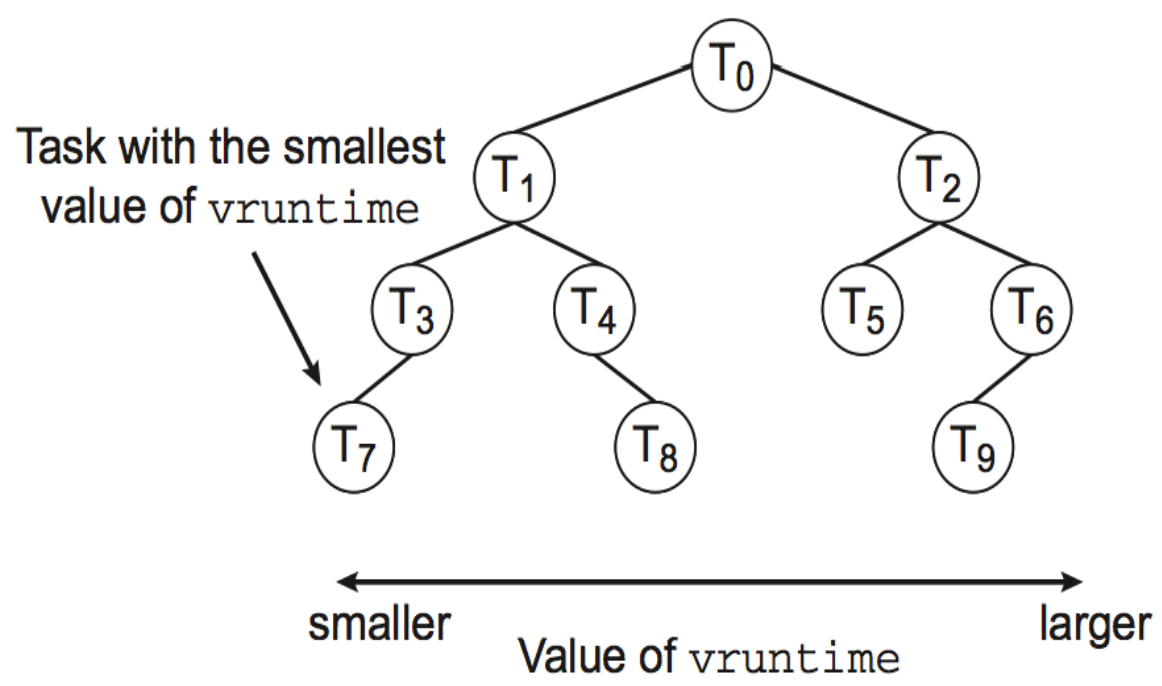
\includegraphics[width=0.5\linewidth]{img/btree.png}
    
    
\end{figure}


\subsection{Windows Scheduling}

Windows uses priority-based preemptive scheduling. Highest-priority thread runs next.
\textbf{Dispatcher} is scheduler.  

Windows has a 32-level priority scheme, where \textbf{Variable class} is 1-15, \textbf{real-time class} is 16-31. Priority 0 is memory-management thread.

It is a multilevel queue for each level and if no run-able thread, it runs \textbf{idle thread} a task that do noting.


\begin{figure}[htbp]
    \centering
    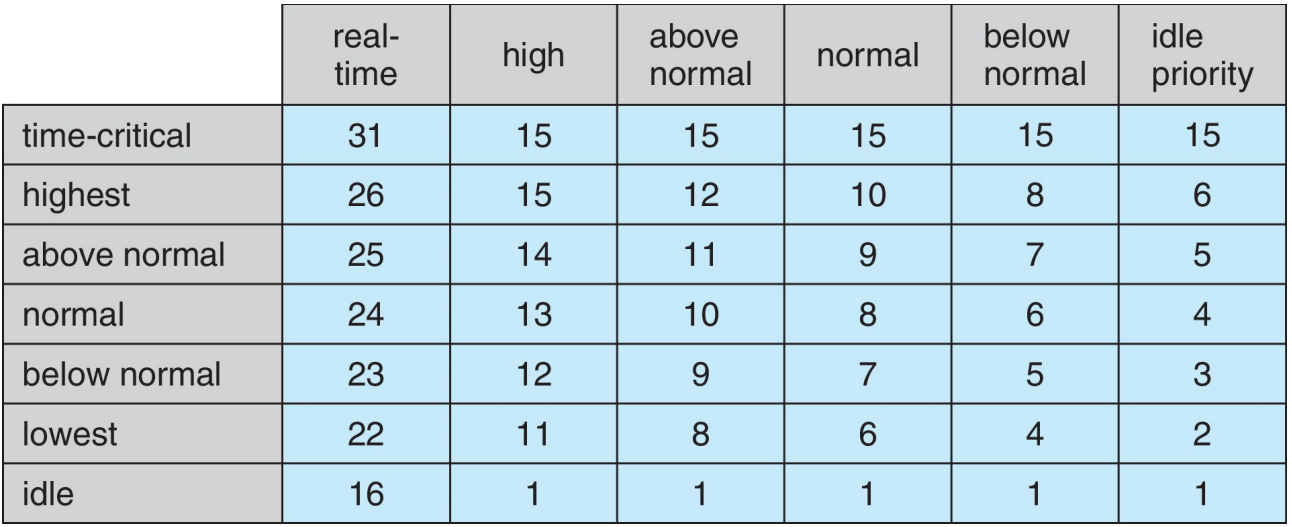
\includegraphics[width=0.7\linewidth]{img/WP.png}
    \caption{Windows priorities}
    
\end{figure}


\subsection{Solaris}

The Solaris OS is used for business. This OS is Priority-based scheduling and has six classes of priority available:


\begin{itemize}
    \item Time sharing (default) (TS)
    \item Interactive (IA)
    \item Real time (RT)
    \item System (SYS)
    \item Fair Share (FSS)
    \item Fixed priority (FP)
\end{itemize}

Given thread can be in one class at a time and  each class has its own scheduling algorithm. Time sharing is multi-level feedback queue, loadable table configurable by sysadmin.

\begin{figure}[htbp]
    \centering
    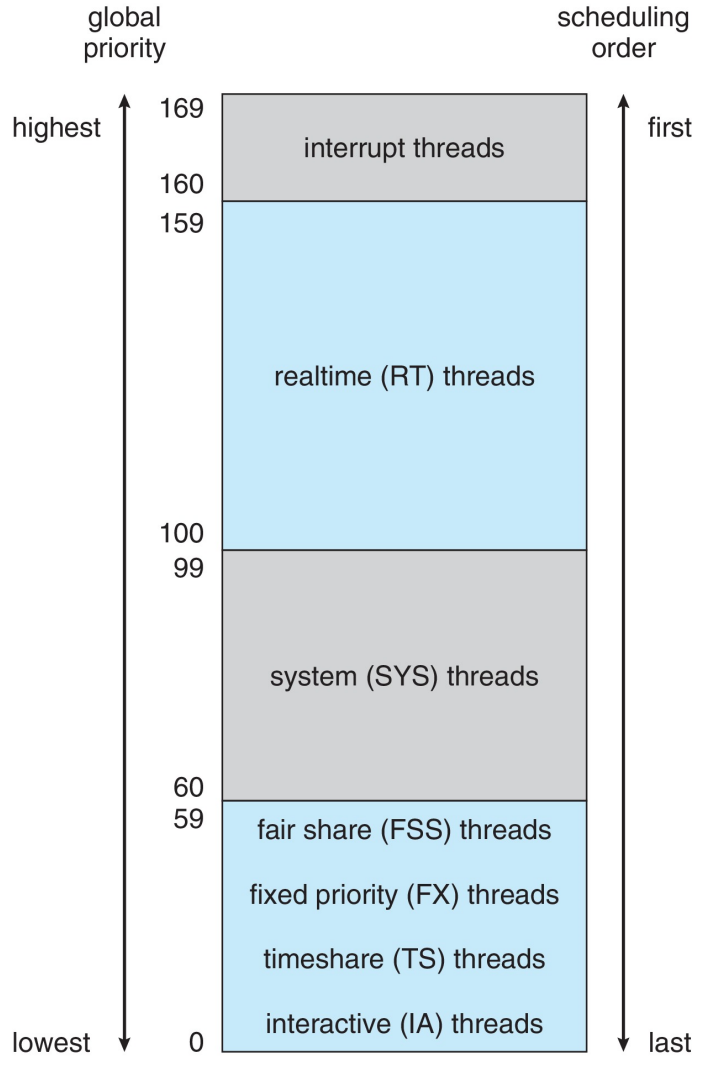
\includegraphics[width=0.4\linewidth]{img/ssolaris.png}
    \caption{Solaris scheduling}
    
\end{figure}

\newpage
\section{Scheduling evaluation}

The scheduling algorithm depends on who is the final users: reading mail, surfing on internet, coding, gaming, render a video, etc. all this tasks required different CPU burst and  we would implement a  \textbf{Deterministic model} to know the CPU burst.

The analytic evaluation is used to takes a particular predetermined workload and defines the performance of each algorithm for that workload.

\subsubsection{Consider 5 processes arriving at time 0:}


\begin{table}[htbp]
    \centering
    \begin{tabular}{cc}
        Processes & Burst Time\\
        \hline
        P1 & 10 \\
        P2 & 29\\
        P3 & 3\\
        P4 & 7\\
        P5 & 12\\
    \end{tabular}
\end{table}

The Deterministic Evaluation for each algorithm, calculate minimum average waiting time, simple and fast, but requires exact numbers for input, applies only to those inputs:

\begin{itemize}
    \item FCS is $28ms$
    \item Non-preemptive SFJ is $13ms$
    \item RR is $23ms$
\end{itemize}


 This deterministic model is not applicable in the real-word.

 \subsection{Queueing models}
Queueing models are mathematical tools used to analyze systems where customers (or items) wait for service. This model describes the arrival of processes, and CPU and I/O bursts probabilistically. These models help predict things like average queue lengths, waiting times, server utilization, and the probability of having a certain number of customers in the system.

Computer system described as network of servers, each with queue of waiting processes

\subsubsection{Little's Formula}

Little’s law – in steady state, processes leaving queue must
equal processes arriving, thus:

\begin{equation*}
    n = \lambda W
\end{equation*}

Where:

\begin{itemize}
    \item[] n = average queue length
    \item[] W = average waiting time in queue
    \item[] $\lambda$ = average arrival rate into queue
\end{itemize}

For example, if on average 7 processes arrive per second, and
normally 14 processes in queue, then average wait time per
process = 2 seconds; but if I have a CPU that can execute only 6 tasks per second the queue grow.


\newpage
\paragraph{Problem: }very rough estimate.

\subsection{Simulations}

Queueing models limited, \textbf{Simulations} more accurate. Is a virtual model, more the model is close to the real behavior and more the simulation is real and the statistics accurate.

Other option is just implement new scheduler and test in the real system, this involves:

\begin{itemize}
    \item High cost, high risk
    \item Environments vary
\end{itemize}

The simulation is one of the possible low cost solution to try new scheduler.
